\section{Schedule classification}

Classify the following schedule with respect to CSR and VSR classes:  
\[r_5(x) r_3(y) w_3(y) r_6(t) r_5(t) w_5(z) w_4(x) r_3(z) w_1(y) r_6(y) w_6(t) w_4(z) w_1(t) w_3(x) w_1(x) r_1(z) w_2(t) w_2(z)\]

\paragraph*{Solution}
Since CSR contains VSR we check with the conflict graph. To do so we first divide the schedule based on the resources: 
\begin{itemize}
    \item $t: \: r_6 \: r_5 \: w_6 \: w_1 \: w_2$
    \item $x: \: r_5 \: w_4 \: w_3 \: w_1$
    \item $y: \: r_3 \: w_3 \: w_1 \: r_6$
    \item $z: \: w_5 \: r_3 \: w_4 \: r_1 \: w_2$
\end{itemize}
The nodes are $\{1,2,3,4,5,6\}$ and the arcs are found with the write-write or write-read relations found in the previous groups. So we have the following graph:
\begin{figure}[H]
    \centering
    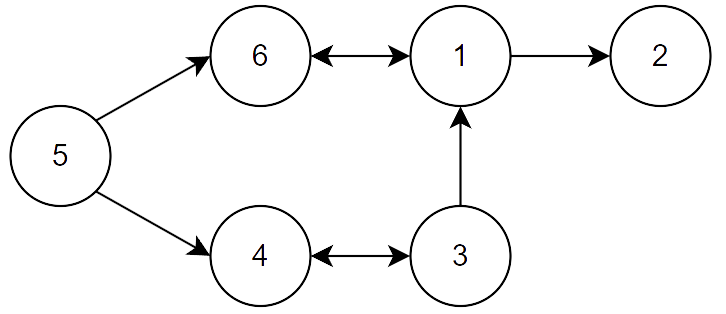
\includegraphics[width=0.5\linewidth]{images/conflictgraph3.png}
\end{figure}
We have two cycles. It is impossible to find a VSR schedule because only the conflict between four and three can be eliminated (the other one changes a read-write relation).